%%%%%%%%%%%%%%%%%%%%%%%%%%%%%%%%%%%%%%%%%%%%%%%%%%%%%%%%%%
%
% Doctoral Thesis Template @ The University of Manchester
% LaTeX Chapter Template
% Version 1 (23/07/2020)
% Joe Crone
%
% This template is based on:
% The University of Manchester, Presentation of Thesis Policy
% Research Office Graduate Education Team
% June 2017
% http://www.regulations.manchester.ac.uk/pgr-presentation-theses/
%
%%%%%%%%%%%%%%%%%%%%%%%%%%%%%%%%%%%%%%%%%%%%%%%%%%%%%%%%%%
\documentclass[../main.tex]{subfiles}
\begin{document}

% Title
%--------------------------------------------------------
\chapter{Optimisation and Characterisation of Inverse Compton Scattering Spectra}
\label{Optimisation_and_Characterisation_of_Inverse_Compton Scattering_Spectra} % to reference use \ref{ChapterTemplate}

\section{Motivation for Characterisation of ICS Sources}

Proper characterisation of inverse Compton scattering sources is necessary to quantify source performance for reliable comparison of sources. Through design and benchmarking of models to predict ICS source performance, understanding of the interaction is gained which can show routes to improving narrowband ICS source design such as the optimisation strategies covered later in this chapter, which were motivated by the characterisation work. Unlike the spectral output parameters presented in Chapter~\ref{Photon_Production_by_Inverse_Compton_Scattering}, which show only a snapshot of source performance, models need to be designed to take into account collimation and account for all necessary effects such as energy spread and emittance effects present in the spectrum. This allows the spectrum of the radiation produced by an ICS source to be predicted and therefore users can understand the experimental probe used in their light source experiments.

Within the first half of this chapter, an analytical approach to calculating the collimated flux produced by an ICS source is developed and compared to existing methods \cite{curatolo2017analytical} and a semi-analytical spectrum code \textsc{ICARUS}: inverse Compton scattering semi-analytical recoil-corrected ultra-relativistic spectrum code based on the model by Sun et al \cite{sun2009characterizations,sun2011theoretical}, which is corrected and expanded, is developed and benchmarked using the \textsc{ICCS3D} code \cite{krafft2016laser,ranjan2018simulation}. The characterisation methods developed here are tested by several cases outlined in Section~\ref{sec:benchmarking_cases_characterisation_optimisation} to encapsulate the range of typical drivers of inverse Compton scattering source, not limiting this work to ERLs alone.

\textcolor{blue}{**WHY DEV AN ANALYTICAL COLLIMATED FLUX \\**}
An analytical collimated flux equation has been developed in Section~\ref{sec:analytical_collimated_flux} in order to provide a quick, reliable method to predict the yield of spectrum codes. Using this method, more accurate simulations such as those from the \textsc{ICAURUS} spectrum code can be evaluated. A wide variety of effects such as collimation, angular crossing and hourglass effects have been incorporated into this methodology, with the notable neglection of the effect of energy spread of the electron bunch and spectral bandwidth of the laser pulse. Large-scale spectrum code simulations require computational time on the order of hours, with parallel computing whereas analytical calculations can be evaluated in sub-second timescales. Therefore, analytical collimated flux calculations are easier to apply to optimisation procedures rather than the more accurate spectral yield calculations from spectrum codes.   

\textcolor{blue}{**WHY CHOSE SEMI-ANALYTICAL MODEL**\\}
The \textsc{ICARUS} spectrum code is a dedicated semi-analytical inverse Compton scattering codes unlike the standard ICS source Monte Carlo simulation code \textsc{CAIN} \cite{chen1995cain}, which simulates electromagnetic interactions with subroutines to limit the code only to the ICS interaction. A semi-analytical ICS spectrum code is advantageous to Monte Carlo based techniques such as the \textsc{CAIN}  spectrum code as  collimation effects aren't taken into account within the simulation and are instead required as part of post-simulation analysis. Because \textsc{CAIN} treats the incident laser pulse as an electric field, the effect of the spectral bandwidth of the pulse isn't properly accounted for which is necessary for the ICS interaction where this can be the main contributor to the bandwidth of the resulting spectrum. Inherently, in Monte Carlo simulation rare events in nature will be as rare in the simulation, therefore statistics in situations where low scattered photon counts are expected are poor; for example in the tails of the distribution, at very narrow apertures \cite{ranjan2018simulation} and in re-circulated ICS sources where low flux interactions are conducted at high repetition rate. 

\section{Analytical Collimated Flux}
\label{sec:analytical_collimated_flux}

In this section, the collimated flux - the total flux collected within an aperture of semi-angle $\theta_{\mathrm{col}}$ is derived from first principles, using the work of Berestetskii et al \cite{berestetskii1982quantum}. This method, unlike others in the literature \cite{curatolo2017analytical}, is valid for the angular crossing case ($\phi\in\mathbb{R}$) as the effect of the crossing angle is encompassed in the cross section alongside the geometric beam--beam angular crossing effect. The hourglass effect is also fully accounted for in this method, using the prescription of Miyahara \cite{miyahara2008luminosity}. The collimated flux calculation method is a semi-analytic calculation that is valid within the recoil regime (above $X\ll1$) but is only valid for the linear inverse Compton scattering case ($a_{0}\ll1$).

In order to find the scattering angle $\theta$ dependence of the cross section \textcolor{blue}{link to cross section derivation/work} we must focus on the dependence of the scattering angle on the Lorentz invariant quantities ($X$ and $Y$) (Eq.~\ref{eq:X_geometry},~\ref{eq:Y_geometry}) derived from Mandelstam variables in Section~\ref{sec:electron_photon_interactions}. Intrinsically, our definition of the recoil parameter $X$ (Eq.~\ref{eq:X_Mandelstam}) relates to the centre of mass $s$ Mandelstam variable before the interaction, so there is no scattering angle  dependence. The $Y$ Lorentx invariant is dependent on $\theta$, to include it's scattering angle dependence we must examine the derivative of $Y$ with $\theta$. Inspecting (Eq.~\ref{eq:Y_geometry}) we see $Y$ is also dependent on $E_{\gamma}$, the scattered photon energy (Eq.~\ref{eq:scattered_photon_energy}) derived in Section~\ref{sec:derivation_of_the_scattered_photon_energy}, which is also dependent on scattering angle. Thus, we must first expand $Y$ which can be simplified in terms of the recoil parameter $X$ (Eq.~\ref{eq:X_geometry})
\begin{equation}
Y = \frac{2\gamma E_{L}\left(1+\beta\cos\phi\right)\left(1-\beta\cos\theta\right)}{m_{e}c^{2}\left\{1-\beta\cos\theta+\left[1+\cos\left(\phi+\theta\right)\right]E_{L}/E_{e}\right\}} = \frac{X\left(1-\beta\cos\theta\right)}{1-\beta\cos\theta+\left[1+\cos\left(\phi+\theta\right)\right]E_{L}/E_{e}}.
\label{eq:Y_geometry_expanded}
\end{equation}
For our purposes, we require the derivative of $Y$ with respect to $\theta$. The derivative of our expanded $Y$ Lorentz invariant (Eq.~\ref{eq:Y_geometry_expanded}) is best found using the quotient rule  
\begin{gather}
Y\left(\theta\right) = \frac{g\left(\theta\right)}{h\left(\theta\right)}, \\
\frac{dY\left(\theta\right)}{d\theta} = \frac{g'\left(\theta\right)h\left(\theta\right)-g\left(\theta\right)h'\left(\theta\right)}{\left[h\left(\theta\right)\right]^{2}},
\label{eq:quotient_rule}
\end{gather}
where the terms in (Eq.~\ref{eq:quotient_rule}) are given by
\begin{gather}
g\left(\theta\right) = X\left(1-\beta\cos\theta\right), \\
g'\left(\theta\right) = X\beta\sin\theta, \\
h\left(\theta\right) = 1-\beta\cos\theta+\left[1+\cos\left(\phi+\theta\right)\right]E_{L}/E_{e}, \\
h'\left(\theta\right) = \beta\sin\theta-\sin\left(\phi+\theta\right)E_{L}/E_{e}.
\label{eq:quotientterms}
\end{gather}
The full derivative of $Y$ by $\theta$ is therefore
\begin{equation}
\frac{dY}{d\theta} = \frac{X\beta\sin\theta\left\{1-\beta\cos\theta+\left[1+\cos\left(\phi+\theta\right)\right]E_{L}/E_{e}\right\}-X\left(1-\beta\cos\theta\right)\left[\beta\sin\theta-\sin\left(\phi+\theta\right)E_{L}/E_{e}\right]}{\left\{1-\beta\cos\theta+\left[1+\cos\left(\phi+\theta\right)\right]E_{L}/E_{e}\right\}^{2}}.
\label{eq:dY_dtheta}
\end{equation}

\begin{figure}[!h]
\centering
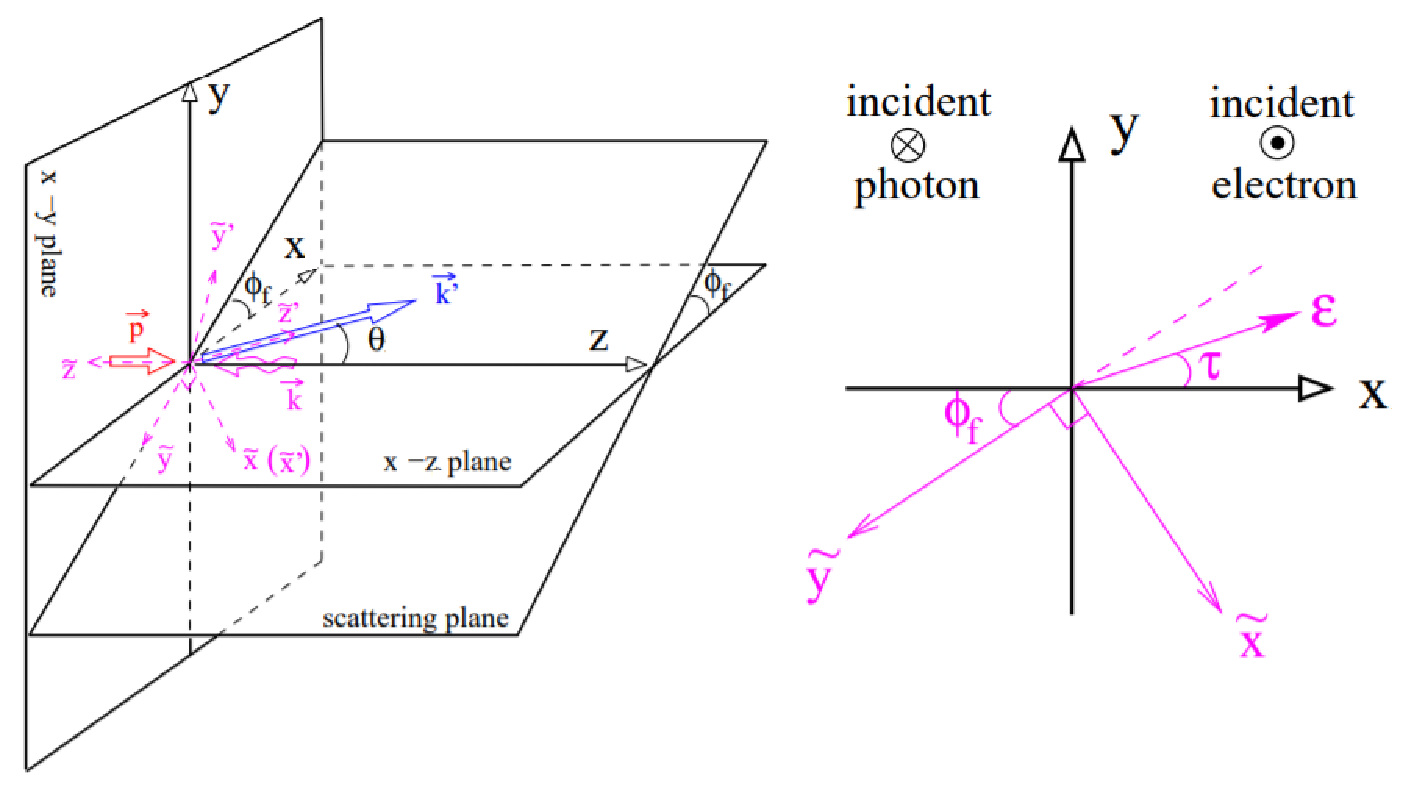
\includegraphics[width=\textwidth]{Figures/Photon_Production_by_Inverse_Compton_Scattering/SunPolarisationScatteringDiagram.pdf}
\caption{Left: The 3D scattering geometry of the electron - photon interaction by C. Sun \cite{sun2009characterizations}. Here $\phi_{f}$ is the azimuthal angle of the scattered photon and $\tilde{x}, \tilde{y}, \tilde{z}$ define the co-ordinate system of the incident electron and the notation is varied $p = p_{1}$, $k = k_{1}$ and $k' = k_{2}$. Right: Interaction polarisation diagram by C. Sun \cite{sun2009characterizations}. Here $\tau$ is the azimuthal angle of the polarization vector $\epsilon$.\textcolor{blue}{**NEED TO REPLACE DIAGRAM**}}
\label{fig:sun_geometry}
\end{figure}

Since we understand that the cross section's \textcolor{blue}{Link to the cross section section} scattering angle dependence is due to the $Y$ Lorentz invariant, as this is constructed from both Lorentz invariants and the $X$ invariant (Eq.~\ref{eq:X_geometry}) which is defined without scattering angle dependence, we must find the dependence of the cross section on the Lorentz invariant $Y$ in order to propagate the full dependencies. \textcolor{blue}{**some of this is required in the cross section section**} Fig.~\ref{fig:sun_geometry} shows the full 3D geometry of the electron - phton interaction, which includes a polarisation diagram. Following Eq. (2.27) by Sun \cite{sun2009characterizations}, we can then use a standard result from QED for the cross section of the interaction of unpolarised electron beam and polarised laser pulse, without considering the post-interaction polarisations \cite{grozin2002complete} \textcolor{blue}{Did this just stay as an arXiv paper?}
\begin{equation}
\frac{d^{2}\sigma}{dYd\phi_{f}} = \frac{4r_{e}^{2}}{X^{2}}\left\{\left(1-\xi_{3}\right)\left[\left(\frac{1}{X}-\frac{1}{Y}\right)^{2}+\frac{1}{X}-\frac{1}{Y}\right]+\frac{1}{4}\left(\frac{X}{Y}+\frac{Y}{X}\right)\right\},
\label{eq:differential_cross_section_Y_phif}
\end{equation}
where $\phi_{f}$ is the azimuthal angle of the scattered photon, $r_{e}$ is the classical electron radius, $X$ and $Y$ are the Lorentz invariants in (Eq.~\ref{eq:X_geometry}, \ref{eq:Y_geometry}) and $\xi_{3}$ is the Stokes parameter, describing linear polarisation aligned to the $x$ or $y$ axis, given by
\begin{equation}
\xi_{3} = -P_{t}\cos\left(2\tau-2\phi_{f}\right),
\label{eq:stokes_3}
\end{equation} 
with $0 \leq P_{t} \leq 1$, the degree of linear polarisation and $\tau$ the azimuthal angle of the polarisation vector. 

We can then integrate over the azimuthal scattering angle $\phi_{f}$
\begin{equation}
\frac{d\sigma}{dY} = \frac{4r_{e}^{2}}{X^{2}}\int_{0}^{2\pi}\left[1+P_{t}\cos\left(2\tau-2\phi_{f}\right)\right]\left\{\left(1-\xi_{3}\right)\left[\left(\frac{1}{X}-\frac{1}{Y}\right)^{2}+\frac{1}{X}-\frac{1}{Y}\right]+\frac{1}{4}\left(\frac{X}{Y}+\frac{Y}{X}\right)\right\} d\phi_{f}, 
\label{eq:phif_integral}
\end{equation}
we can then take the case of an unpolarised laser pulse or a circularly polarised laser pulse ($P_{t} = 0$), or acknowledge that this polarisation term becomes zero once integrated over the full azimuthal angle $\phi_{f}$, to simplify this to
\begin{equation}
\frac{d\sigma}{dY} = \frac{8\pi r_{e}^{2}}{X^{2}}\left\{\left[\left(\frac{1}{X}-\frac{1}{Y}\right)^{2}+\frac{1}{X}-\frac{1}{Y}\right]+\frac{1}{4}\left(\frac{X}{Y}+\frac{Y}{X}\right)\right\},
\label{eq:cross_section_Y_berestetskii_form}
\end{equation}
which replicates the form in Eq. (86.16) by Berestetskii et al \cite{berestetskii1982quantum}.

The dependence of the cross section $\sigma$ upon the scattering angle $\theta$ can be found using the chain rule
\begin{equation}
\frac{d\sigma}{d\theta} = \frac{d\sigma}{dY}\frac{dY}{d\theta}.
\label{eq:cross_section_chain_rule}
\end{equation}
Therefore, the cross section for a collimation angle $\theta_{\mathrm{col}}$ becomes
\begin{equation}
\sigma\left(\theta_{\mathrm{col}}\right) = \int_{0}^{\theta_{\mathrm{col}}}\frac{d\sigma}{dY}\frac{dY}{d\theta}d\theta,
\label{eq:cross_section_integral}
\end{equation} 
where $\frac{d\sigma}{dY}$ is given by (Eq.~\ref{eq:cross_section_Y_berestetskii_form}) and $\frac{dY}{d\theta}$ is given by (Eq.~\ref{eq:dY_dtheta}). The full cross section calculation is summarised as
\begin{multline}
\sigma\left(\theta_{\mathrm{col}}\right) = \int_{0}^{\theta_{\mathrm{col}}} \frac{8\pi r_{e}^{2}}{X^{2}}\left\{\left[\left(\frac{1}{X}-\frac{1}{Y}\right)^{2}+\frac{1}{X}-\frac{1}{Y}\right]+\frac{1}{4}\left(\frac{X}{Y}+\frac{Y}{X}\right)\right\}\\\frac{X\beta\sin\theta\left\{1-\beta\cos\theta+\left[1+\cos\left(\phi+\theta\right)\right]E_{L}/E_{e}\right\}-X\left(1-\beta\cos\theta\right)\left[\beta\sin\theta-\sin\left(\phi+\theta\right)E_{L}/E_{e}\right]}{\left\{1-\beta\cos\theta+\left[1+\cos\left(\phi+\theta\right)\right]E_{L}/E_{e}\right\}^{2}}d\theta,
\label{eq:full_scattering_angle_cross_section_integral}
\end{multline}
where $Y, X, E_{\gamma}$ are of the forms in (Eq.~\ref{eq:Y_geometry},~\ref{eq:X_geometry},~\ref{eq:scattered_photon_energy}). Using the results derived in Sections~\ref{sec:luminosity_and_flux},~\ref{sec:angular_crossing_and_hourglass_effects} the collimated flux is given by a modified cross section (Eq.~\ref{eq:full_scattering_angle_cross_section_integral}) form of the flux equation (Eq.~\ref{eq:headon_flux}), with an angular crossing and the  hourglass effect taken into account (Eq.~\ref{eq:flux_angular_crossing_hourglass})
\begin{equation}
\mathcal{F}_{\mathrm{col}} = \sigma\left(\theta_{\mathrm{col}}\right) R_{ACHG}\mathcal{L}_{\mathrm{HEAD-ON}}f.
\label{eq:collimated_flux}
\end{equation}

It is inherent in (Eq.~\ref{eq:collimated_flux}) that the interaction occurs from a point source - the transverse and longitudinal positions of the electrons within the bunch are neglected. This is a common approximation in both simulations and in all presented flux formulae.

Within (Eq.~\ref{eq:collimated_flux}) the effect of the energy spread of the bunch, the laser pulse energy spread (spectral bandwidth) and partially, via the point source approximation, the effect of the emittance (spatial extent) of the bunch are neglected. The geometry consideration of the spatial extent of the bunch is taken into account via the luminosity reduction factors, but not the offset in emission position which would affect whether the photon passes the collimator. The codes \textsc{ICARUS} and \textsc{ICCS3D} \cite{krafft2016laser,ranjan2018simulation} properly take into account the energy spread factors but the emission position problem is only solved in Monte Carlo codes such as \texsc{CAIN} \cite{chen1995cain}. However, this effect is expected to be small as the source is dependent on far-field collimation. Far-field collimation is applicable when the transverse size of the electron bunch - laser pulse overlap is negligible in relation to the aperture of the collimator. 

\section{Development of the ICARUS Spectrum code}
\label{sec:development_of_the_ICARUS_spectrum_code}

\textcolor{blue}{**USE $\sim$ BETWEEN INTEGRATION VARIABLES FOR PROPER SPACING**}

Using the result of Sun et al \cite{sun2009characterizations,sun2011theoretical}, the spatial and energy distributions of a $\gamma$-ray beam produced by a head-on collision of an electron bunch and laser pulse is given by
\begin{multline}
\frac{dN_{\gamma}}{d\Omega_{d} dE_{\gamma}} = N_{e}N_{L}\int \frac{d\sigma}{d\Omega}\delta\left(\bar{E_{\gamma}}-E_{\gamma}\right)c\left(1+\beta\right)f_{e}\left(x,y,z,x',y',p,t\right)\\ \times f_L\left(x,y,z,k,t\right)dx'~dy'~dp~dk~dV~dt,
\label{eq:central_distribution_sun}
\end{multline}
where the detection solid angle is $d\Omega = dx_{d}dy_{d}/L^{2}$ with $x_{d}$ and $y_{d}$ the $x$ and $y$ positions at the detector and $L$ the source-to-detector distance, $\frac{d\sigma}{d\Omega}$ is the differential cross section of the ICS interaction, $\delts\left(\bar{E_{\gamma}}-E_{\gamma}\right)$ is a delta function which encapsulates energy conservation in the process with $\bar{E_{\gamma}}$ the maximum possible energy a $\gamma$-ray have for a scattering angle $\theta$ and $E_{\gamma}$ the actual $\gamma$-ray energy, the $c\left(1+\beta\right)$ term arises from the Doppler shifting of the radiation, $f_{e}$ and $f_{L}$ are the phase-space intensity distributions of the electron bunch (Eq.~\ref{eq:electron_gaussian_intensity_distribution}) and laser pulse (Eq.~\ref{eq:laser_gaussian_intensity_distribution}) as modelled by Gaussian distributions, $dx'$ and $dy'$ are the divergence integration variables in $x$ and $y$ respectively, $dp$ is momentum of the electron integration variable, $dk$ is the wavenumber of the laser pulse integration variable, $dV$ is the volume of the interaction integration parameter and  $dt$ is the interaction time integration variable. 

The differential cross section for a head-on collision in this model is given by
\begin{equation}
\frac{d\sigma}{d\Omega} = 8r_{e}^{2}\left\{\frac{1}{4}\left[\frac{4\gamma^{2}E_{L}}{\bar{E_{\gamma}}\left(1+\gamma^{2}\theta^{2}\right)}+\frac{\bar{E_{\gamma}}\left(1+\gamma^{2}\theta^{2}\right)}{4\gamma^{2}E_{\gamma}}\right]-2\cos^{2}\left(\tau-\phi_{f}\right)\frac{\gamma^{2}\theta^{2}}{\left(1+\gamma^{2}\theta^{2}\right)^{2}}\right\}\left(\frac{\bar{E_{\gamma}}}{4\gamma E_{L}}\right)^{2},
\label{eq:sun_differential_cross_section}    
\end{equation}
where $\bar{E_{\gamma}}$ is the Compton edge energy for a particular scattering angle $\theta$ in the small angle approximation for a head-on ($\phi=0$) collision
\begin{equation}
\bar{E_{\gamma}} = \frac{4\gamma^{2}E_{L}}{1+\gamma^{2}\theta^{2}+\frac{4\gamma E_{L}}{m_{e}c^{2}}}.
\label{eq:sun_Egamma_bar}    
\end{equation}
We can then express the angular divergences $x'$ and $y'$ by the projection of the scattering angle of of the produced radiation in each plane $\theta_{x}'$ and $\theta_{y}'$ ($\theta = \sqrt{\theta_{x}^{2}+\theta_{y}^{2}}$), whilst neglecting the very small angular divergences of the laser pulse, using the relations
\begin{align}
\theta_{x}' + x' &= \frac{x_{d}-x}{L} \\
\theta_{y}' + y' &= \frac{y_{d}-y}{L}
\label{eq:sun_angular_divergence}    
\end{align}
which arise from the geometric constraints of a photon passing through a collimator and impinging on a detector in far-field collimation ($L \gg \sqrt{x_{d}^{2}+y_{d}^{2}}$), where $x$ and $y$ are the positions of the interaction in each plane. We typically assume $x=y=0$ because we assume a point source. Applying (Eq.~\ref{eq:sun_angular_divergence}) and integrating (Eq.~\ref{eq:central_distribution_sun}) with respect to $dV$, the interaction geometric volume and $dt$ the interaction time, whilst expanding the detector solid angle and the Gaussian intensity distributions of the electron bunch (Eq.~\ref{eq:electron_gaussian_intensity_distribution}) and laser pulse (Eq.~\ref{eq:laser_gaussian_intensity_distribution}), we gain
\begin{multline}
\frac{dN_{\gamma}}{dE_{\gamma}dx_{d}dy_{d}} = \frac{N_{e}N_{L}}{\left(2\pi\right)^{3}z_{R}\sigma_{p}\sigma_{k}}\int \frac{k}{\sqrt{\zeta_{x}\zeta_{y}}\sigma_{\theta_{x}}\sigma_{\theta_{y}}}\frac{d\sigma}{d\Omega}\delta\left(\bar{E_{\gamma}}-E_{\gamma}\right)\left(1+\beta\right) \\\times\exp\left[-\frac{\left(\theta_{x}-x_{d}/L\right)^{2}}{2\sigma_{\theta_{x}}^{2}}-\frac{\left(\theta_{y}-y_{d}/L\right)^{2}}{2\sigma_{\theta_{y}}^{2}}-\frac{\left(p-p_{0}\right)^{2}}{2\sigma_{p}^{2}}-\frac{\left(k-k_{0}\right)^{2}}{2\sigma_{k}^{2}}\right]~d\theta_{x}~d\theta_{y}~dp~dk,
\label{eq:sun_volume_time_integral}    
\end{multline}
where $z_{R}$ is the Rayleigh range \textcolor{blue}{**reference once sorted Compton theory**}, the $\zeta_{x/y}$, $\sigma_{\theta_{x/y}}$ and  $\xi_{x/y}$ parameterisations in each plane are given by
\begin{align}
\zeta_{x} &= 1+\frac{2k\beta_{x}\epsilon_{x}}{z_{R}}, & \sigma_{\theta_{x}} &= \sqrt{\frac{\epsilon_{x}\xi_{x}}{\beta_{x}\zeta_{x}}}, & \xi_{x} &= 1+\left(\alpha_{x}-\frac{\beta_{x}}{L}\right)^{2}+\frac{2k\beta_{x}\epsilon_{x}}{z_{R}}, \nonumber\\
\zeta_{y} &= 1+\frac{2k\beta_{y}\epsilon_{y}}{z_{R}}, & \sigma_{\theta_{y}} &= \sqrt{\frac{\epsilon_{y}\xi_{y}}{\beta_{y}\zeta_{y}}}, & \xi_{y} &= 1+\left(\alpha_{y}-\frac{\beta_{y}}{L}\right)^{2}+\frac{2k\beta_{y}\epsilon_{y}}{z_{R}}, 
\label{eq:zeta_sigmatheta_xi_parameters_sun}
\end{align}
where $p_{0}$ is the centroid momentum of the electron bunch and $k_{0}$ is the centroid wavenumber of the laser pulse. Here note that there is an algebraic error in Sun et al's \cite{sun2009characterizations,sun2011theoretical} derivation, the prefactor gives that $dN/dE\propto L^{2}$ for a source-to-detector distance $L$. This arises due to a mishandling of the detector solid angle. Clearly, this should be $dN/dE\propto 1/L^{2}$, meaning there is an inverse square relationship between source-to-detector distance and the spectral density as would be expected. 

The delta function, encompassing the energy conservation of this process can be re-wrote in terms of the Lorentz factor
\begin{equation}
\delta\left(\right) = -\delta\left(\gamma-\bar{\gamma}\right)\frac{\left(1+\right)}{}
\label{sun_electron_energy_delta_function}    
\end{equation}

\begin{multline}
\frac{dN_{\gamma}}{dE_{\gamma}} = \frac{r_{e}^{2}N_{e}N_{L}}{4\pi^{3}L^{2}\hbar c z_{R}\sigma_{\gamma}\sigma_{k}}\int_{k_{\mathrm{min}}}^{k_{\mathrm{max}}}\int_{-\theta_{x,\mathrm{max}}}^{\theta_{x,\mathrm{max}}}\int_{-\theta_{y,\mathrm{max}}}^{\theta_{y,\mathrm{max}}}\int_{y_{\mathrm{min}}}^{y_{\mathrm{max}}}\int_{x_{\mathrm{min}}}^{x_{\mathrm{max}}}\frac{1}{\sqrt{\zeta_{x}\zeta_{y}}\sigma_{\theta_{x}}\sigma_{\theta_{y}}}\frac{\bar{\gamma}}{1+2\gamma E_{L}/m_{e}c^{2}} \\
\times\left\{\frac{1}{4}\left[\frac{4\bar{\gamma}^{2}E_{L}}{E_{\gamma}\left(1+\bar{\gamma}^{2}\theta^{2}\right)}+\frac{E_{\gamma}\left(1+\bar{\gamma}^{2}\theta^{2}\right)}{4\bar{\gamma}^{2}E_{L}}\right]-2\cos^{2}\left(\tau-\phi_{f}\right)\frac{\bar{\gamma}^{2}\theta^{2}}{\left(1+\bar{\gamma}^{2}\theta^{2}\right)^{2}}\right\} \\
\times\exp{\left[-\frac{\left(\theta_{x}-x_{d}/L\right)^{2}}{2\sigma_{\theta_{x}}^{2}}-\frac{\left(\theta_{y}-y_{d}/L\right)^{2}}{2\sigma_{\theta_{y}}^{2}}-\frac{\left(\bar{\gamma}-\gamma\right)^{2}}{2\sigma_{\gamma}^{2}}-\frac{\left(k-k_{0}\right)^{2}}{2\sigma_{k}^{2}}\right]}dx_{d}~dy_{d}~d\theta_{y}~d\theta_{x}~dk,
\label{eq:ICARUS_equation}
\end{multline}







\begin{gather}
\theta_{x,\mathrm{max}} = \sqrt{\frac{4E_{L}}{E_{\gamma}}-\theta_{y}^{2}}, \\
\theta_{y,\mathrm{max}} = \sqrt{\frac{4E_{L}}{E_{\gamma}}},
\label{eq:theta_max_parameter_sun}
\end{gather}

\begin{equation}
\sigma_{\gamma} = \frac{\sigma_{e}}{m_{e}c^{2}},
\label{eq:gamma_energy_spread}
\end{equation}

\begin{equation}
\theta = \sqrt{\theta_{x}^{2}+\theta_{y}^{2}},
\label{eq:theta_angle_sun}
\end{equation}

\begin{equation}
\bar{\gamma} = \frac{2E_{\gamma}E_{L}/m_{e}c^{2}}{4E_{L}-E_{\gamma\theta^{2}}}\left[1+\sqrt{\frac{4E_{L}-E_{\gamma}\theta^{2}}{4E_{L}E_{\gamma}/\left(m_{e}c^{2}\right)^{2}}}\right],  
\label{eq:gamma_bar_sun}
\end{equation}

\begin{multline}
\frac{dN_{\gamma}}{dE_{\gamma}} \approx \frac{r_{e}^{2}N_{e}N_{L}}{2\pi^{2}L^{2}\hbar c z_{R}\sqrt{\zeta_{x}}\sigma_{\gamma}\sigma_{\theta_{x}}}\int_{-\theta_{x,\mathrm{max}}}^{\theta_{x,\mathrm{max}}}\int_{y_{\mathrm{min}}}^{y_{\mathrm{max}}}\int_{x_{\mathrm{min}}}^{\mathrm{max}}\frac{\bar{\gamma}}{1+2\gamma E_{L}/m_{e}c^{2}} \\
\times\left\{\frac{1}{4}\left[\frac{4\bar{\gamma}^{2}E_{L}}{E_{\gamma}\left(1+\bar{\gamma}^{2}\theta^{2}\right)}+\frac{E_{\gamma\left(1+\bar{\gamma}^{2\theta^{2}}\right)}}{4\bar{\gamma}^{2}E_{L}}\right]-\frac{\bar{\gamma}^{2}\theta^{2}}{\left(1+\bar{\gamma}^{2}\theta^{2}\right)^{2}}\right\} \\
\times\exp{\left[-\frac{\left(\theta_{x}-x_{d}/L\right)^{2}}{2\sigma_{\theta_{x}}^{2}}-\frac{\left(\bar{\gamma}-\gamma\right)^{2}}{2\sigma_{\gamma}^{2}}\right]}d\theta_{x}dy_{d}dx_{d},
\label{eq:1D_sun_equation}    
\end{multline}
    
\begin{equation}
\theta_{x,\mathrm{max}} = \sqrt{\frac{4E_{L}}{E_{\gamma}}-\left(\frac{y_{d}}{L}\right)^{2}},
\label{eq:theta_max_parameter_1D_sun}
\end{equation}

\section{Benchmarking Cases for Characterisation and Optimisation}
\label{sec:benchmarking_cases_characterisation_optimisation}

\section{Benchmarking of Characterisation Methods}
\label{sec:benchmarking_of_the_ICARUS_spectrum_code}

\textcolor{blue}{Mention that the Curatolo formula is deficient as it doesn't provide adequate derivation to verify, seemingly that the bandwidth it is based upon is deficient (Ranjan et al say so in (2018), Fig.~1) and doesn't provide angular case either.}

The code \textsc{ICCS3D}, a generalization of the \textsc{ICCS} code \cite{krafft2016laser,ranjan2018simulation}, computes radiation produced in ICS within the linear Compton regime (when $a_{0}\ll 1$, and electron recoil is properly accounted for). In \textsc{ICCS3D}, a 3D laser pulse model replaces the 1D plane wave model used in \textsc{ICCS}. This modification is implemented in a manner described in Terzi\'c et al \cite{terzic2019improving}; instead of all electrons experiencing the same laser field strength $a_{0}$, as they do for a 1D plane wave, their effective laser field strength is dependent on the electron's distance from the laser's center at the moment of scattering. To calculate anticipated spectral output, \textsc{ICCS3D} can use either the parameters of the electron beam or an arbitrary electron distribution, in addition to the laser parameters. For Fig.~\ref{fig:cbetaspectrumplot}, a particle distribution was tracked by \textsc{Tao} \cite{TaoManual} through the bypass lattice to the IP; the distribution at the IP was provided to \textsc{ICCS3D}. When compared to the spectrum calculated using only the electron beam parameters, the differences were negligible. 



\textsc{ICARUS}: inverse Compton scattering semi-analytic recoil-corrected ultra-relativistic spectrum code, uses a modified and corrected  version of the 2D formalism of Sun et al. \cite{sun2011theoretical}. \textsc{ICARUS} integrates the photons at small energy intervals that pass through a given 2D collimator aperture (here circular) for the fundamental laser mode. This code assumes that the electron bunch has a 3D Gaussian distribution, approximates the laser as a 3D Gaussian pulse, and is currently only valid for the head-on ($\phi = 0$) geometry; it has been validated against \textsc{ICCS3D} as well as the analytical results of this paper

\section{Motivation for Optimisation of ICS Sources}

\section{Transverse Profile Matching}

In the literature \cite{akagi2016narrow,deitrick2018high,jacquet2015radiation} \textcolor{blue}{add more examples, BriXS?}, many inverse Compton scattering sources have attempted to maximise flux output via matching the \textit{rms} spot size of the transverse profile of the laser pulse to that of the electron bunch ($\sigma_{L}\approx\sigma_{\mathrm{electron}}$). Here, we term this the transverse profile matching scheme. The transverse profile matching scheme ignores the full interaction dynamics at the IP in favour of a simplistic solution. 

The intensity of the laser and electron bunch are often non-uniform transversely within the bunch or pulse (for example in a Gaussian laser pulse), and instead intensity peaks at the centroid. A laser pulse used in inverse Compton scattering is typically more intense by orders of magnitude than the electron bunch ($N_{L} \gg N_{e}$), for example a 1~\si{\nano\coulomb} bunch contains $N_{e} = 6.25\times 10^{9}$ electrons in comparison to a paltry 1~\si{\micro\joule} Nd:YAG ($\lambda = 1064$~\si{\nano\meter}) laser pulse which contains $N_{L} = 5.35\times 10^{12}$ photons. Therefore, to maximise the probability of electron--photon interaction it is favourable to obey the condition $\sigma_{L} > \sigma_{\mathrm{electron}}$.

To first order, the transverse profile matching scheme is a decent approximation for small crossing angles, laser pulse profiles chosen to avoid the worst diffraction effects and near-round transverse profiles ($\sigma_{L}\sim\sigma_{\mathrm{electron}}$); approximate to electron bunches delivered by an ERL or linac. Within experimental tolerances transverse profile matching may be the most attractive scenario however, for ICS light source operation, high flux narrow-bandwidth operation is necessary and optimisation of transverse interaction point parameters can improve this. 

\textcolor{blue}{**Would benefit from some kind of example calculation**}

\section{1D Round Beam Optimisation}
\label{sec:RB_optimisation}

The bandwidth of an ICS light source is tuneable and can be selected on the basis of user requirements. Here we develop a method to maximise flux within a selected \textit{rms} bandwidth for the simplified case of an electron beam with a round transverse profile i.e normalised emittance is identical in both directions ($\epsilon_{nx} = \epsilon_{ny} = \epsilon_{n}$). This can simply be converted to a FWHM bandwidth (Eq.~\ref{eq:FWHM_bandwidth}). Bandwidth selection is possible by selecting $\beta^{*}$ at the IP and by setting the collimation angle, $\theta_{\mathrm{col}}$ that collects the scattered photons; these may for example comprise switchable, fixed-aperture collimators.

Within this optimisation derivation, the \textit{rms} bandwidth is given by (Eq.~\ref{eq:RMS_bandwidth}) with the emittance term (Eq.~\ref{eq:emittance_term}) modified for the transversely round bunch case
\begin{equation}
\frac{\sigma_{\epsilon}}{E_{\epsilon}} = \frac{2\gamma\epsilon_{n}}{\left(1+X\right)\beta^{*}},
\label{eq:emittance_term_round_beam}    
\end{equation}
where $X$ is the recoil parameter (Eq.~\ref{eq:X_geometry}), $\epsilon_{n}$ is the transverse \textit{rms} normalised emittance of the electron bunch and $\beta^{*}$ is the $\beta$-function at the interaction point.

Typically the dominant terms that define the bandwidth of an inverse Compton source Eq.~(\ref{eq:RMS_bandwidth}) are the collimation term Eq.~(\ref{eq:collimation_term}) and the emittance term Eq.~(\ref{eq:emittance_term_round_beam}). The free parameter of the collimation term is the collimation angle $\theta_{\mathrm{col}}$, which can be adjusted either by changing the collimator aperture or changing its distance from the IP. Adjustable collimators have been designed for the ELI-NP-GBS $\gamma$-ray ICS source~\cite{paterno2017collimation}; a similar design could be implemented at other ICS sources.

The emittance term is dependent both on the normalised transverse emittance $\epsilon_{n}$ and on $\beta^{*}$. It is more convenient to change the $\beta$-function at the IP with focusing rather than by varying the emittance, since the latter is dependent on the injector and collective effects prior to the IP. By using a larger $\beta^{*}$ and a small collimator aperture, it is possible to reduce the contribution of the collimation and emittance terms so that they are negligible; thus the electron bunch and laser pulse energy spread terms (Eq.~\ref{eq:beam_energy_spread_term},~\ref{eq:laser_energy_spread_term}) become dominant for accelerators with a sufficiently small emittance. This effectively places a lower limit on the bandwidth of an ICS source, i.e. it is limited by the energy spread of the electron beam $\Delta E_{e}/E_{e}$ and laser pulse $\Delta E_{\mathrm{laser}}/E_{\mathrm{laser}}$ as 
\begin{equation}
\left(\frac{\Delta E_{\gamma}}{E_{\gamma}}\right)_{\mathrm{min}} \approx \sqrt{\left[\left(\frac{2+X}{1+X}\right)\frac{\Delta E_{e}}{E_{e}}\right]^{2} + \left[\left(\frac{1}{1+X}\right)\frac{\Delta E_{L}}{E_{L}}\right]^{2}},
\label{eq:bandwidth_limitation_minimum}
\end{equation}
for the low recoil approximation.

Consequently, any bandwidth above this limit can be achieved by an ICS source by tuning of the collimation angle and $\beta^*$ so that a desired bandwidth, $\Delta E_{\gamma}/E_{\gamma}$, is achieved. Since the collimation and emittance terms are typically dominant, all other terms can be excluded and the solutions are bounded by
\begin{equation}
\frac{\Delta E_{\gamma}}{E_{\gamma}} > \sqrt{\left(\frac{ \sigma_{\theta}}{E_{\theta}}\right)^{2}+\left(\frac{\sigma_{\epsilon}}{E_{\epsilon}}\right)^{2}}.    
\end{equation}
This results in myriad combinations of $\beta^{*}$ and $\theta_{\mathrm{col}}$ that satisfy a particular chosen bandwidth larger than this lower limit (Eq.~\ref{eq:bandwidth_limitation_minimum}).

The different $\beta^{*}$, $\theta_{\mathrm{col}}$ combinations each give a different collimated flux; obviously we wish to chose the solution with the largest flux. The collimated flux $\mathcal{F}_{\Psi}$ of each solution is calculated based on a method valid for small collimation angles ($\gamma\theta_{\mathrm{col}} < 1$) derived by Curatolo et al.~\cite{curatolo2017analytical}. Re-cast for our variable definitions, it becomes
\textcolor{blue}{**THIS MAY CHANGE WITH THE NEW COLLIMATED FLUX METHOD**}
% serafini calc
\begin{equation}
\mathcal{F}_{\Psi}\propto \frac{\left(1+\sqrt[3]{X}\Psi^{2}/3\right)\Psi^{2}}{\left[1+\left(1+X/2\right)\Psi^{2}\right]\left(1+\Psi^{2}\right)}, 
\label{eq:curatolo_collimated_flux}
\end{equation}
where $\mathcal{F}$ is the total (uncollimated) flux, $\Psi = \gamma\theta_{\mathrm{col}}$ is the acceptance angle, and $X$ is the recoil parameter. The solution giving the maximal flux is selected.

It is not practicable to calculate the flux from every combination of $\beta^{*}$ and $\theta_{\mathrm{col}}$. Instead, an array of collimation angles $\theta_{\mathrm{col}}$ from 0 to $1/\gamma$ is used ($\gamma\theta_{\mathrm{col}}<1$), and for a given \textit{rms} bandwidth value the corresponding $\beta^*$ is calculated using
\begin{equation}
\beta^{*} = \frac{2\gamma\epsilon_{n}}{\left(1+X\right)\sqrt{\left(\frac{\Delta E_{\gamma}}{E_{\gamma}}\right)^{2}-\left[\left(\frac{\sigma_{\theta}}{E_{\theta}}\right)^{2}+\left(\frac{\sigma_{e}}{E_{e}}\right)^{2}+\left(\frac{\sigma_{L}}{E_{L}}\right)^{2}\right]}},
\label{eq:beta_star_round_beam}
\end{equation}
which is a rearrangement of (Eq.~\ref{eq:RMS_bandwidth}) with the emittance term in the transversely round bunch case (Eq.~\ref{eq:emittance_term_round_beam}). A near identical solution can also be found for the case of an FWHM bandwidth. 

The collimated flux $\mathcal{F}_{\Psi}$ is calculated for each combination produced via this method. The maximal collimated flux is selected and the combination of $\beta^{*}$ and $\theta_{\mathrm{col}}$ corresponding to this solution is returned. This process can be applied to the case of a target bandwidth to determine $\theta_{\mathrm{col}}$, $\beta^{*}$, and collimated flux in the selected bandwidth. In addition, applying this method to a continuum of bandwidths allows us to map the possible operational settings of our ICS source, and to derive tuning curves such as the variation of the collimated flux with bandwidth.

\section{2D Non-Round Beam Optimisation}

\subsection{Genetic Algorithm Approach}

\subsection{Nelder--Mead Approach}

\section{Evaluation of Optimisation Methods} 

 

\end{document}